\documentclass[tikz,border=10pt]{standalone}
% Shared preamble for the CenterTask panel files (panel_a/b/c.tex).
% Edit colours and node styles here, once.
\usepackage{amsmath}
\usetikzlibrary{arrows.meta,positioning,calc}

% category colours as in ColorCategoryMap.m: 1=Short/Orange, 2=Mid/Green, 3=Long/Blue
\definecolor{catShort}{RGB}{243,178,132}
\definecolor{catMid}{RGB}{158,209,172}
\definecolor{catLong}{RGB}{157,188,234}

\tikzset{ctpanel/.style={
  font=\sffamily,
  band/.style={rounded corners=6pt, fill=black!7, draw=none, inner sep=8pt, minimum height=1.15cm},
  unit/.style={circle, fill=catMid!60, draw=none, minimum size=0.95cm, inner sep=0pt},
  flow/.style={-{Latex[length=2.2mm]}, line width=0.8pt},
  rowlab/.style={anchor=east, font=\sffamily\large},
  now/.style={fill=catShort!55, rounded corners=3pt, inner sep=3pt},
  stage/.style={rounded corners=6pt, fill=black!8, draw=none, inner sep=8pt, minimum height=1.2cm, align=center},
  target/.style={circle, minimum size=0.9cm, inner sep=0pt, draw=none, font=\sffamily\scriptsize, text=black!75},
  axis/.style={line width=0.6pt},
}}


% ---------------------------------------------------------------------
%  Trial-level tiny RNN: two ways of knowing the rule (2 vs 3 categories).
%  Left : the cue (2 or 3 dots) is an input -> the rule switches in one trial.
%  Right: no cue input -> the hidden state must infer the rule from feedback.
%  Both read out the same way: two criteria c1, c2 on the length axis. In
%  3-cat they sit apart (5.05, 6.40); in 2-cat they collapse onto 5.85.
% ---------------------------------------------------------------------

\begin{document}
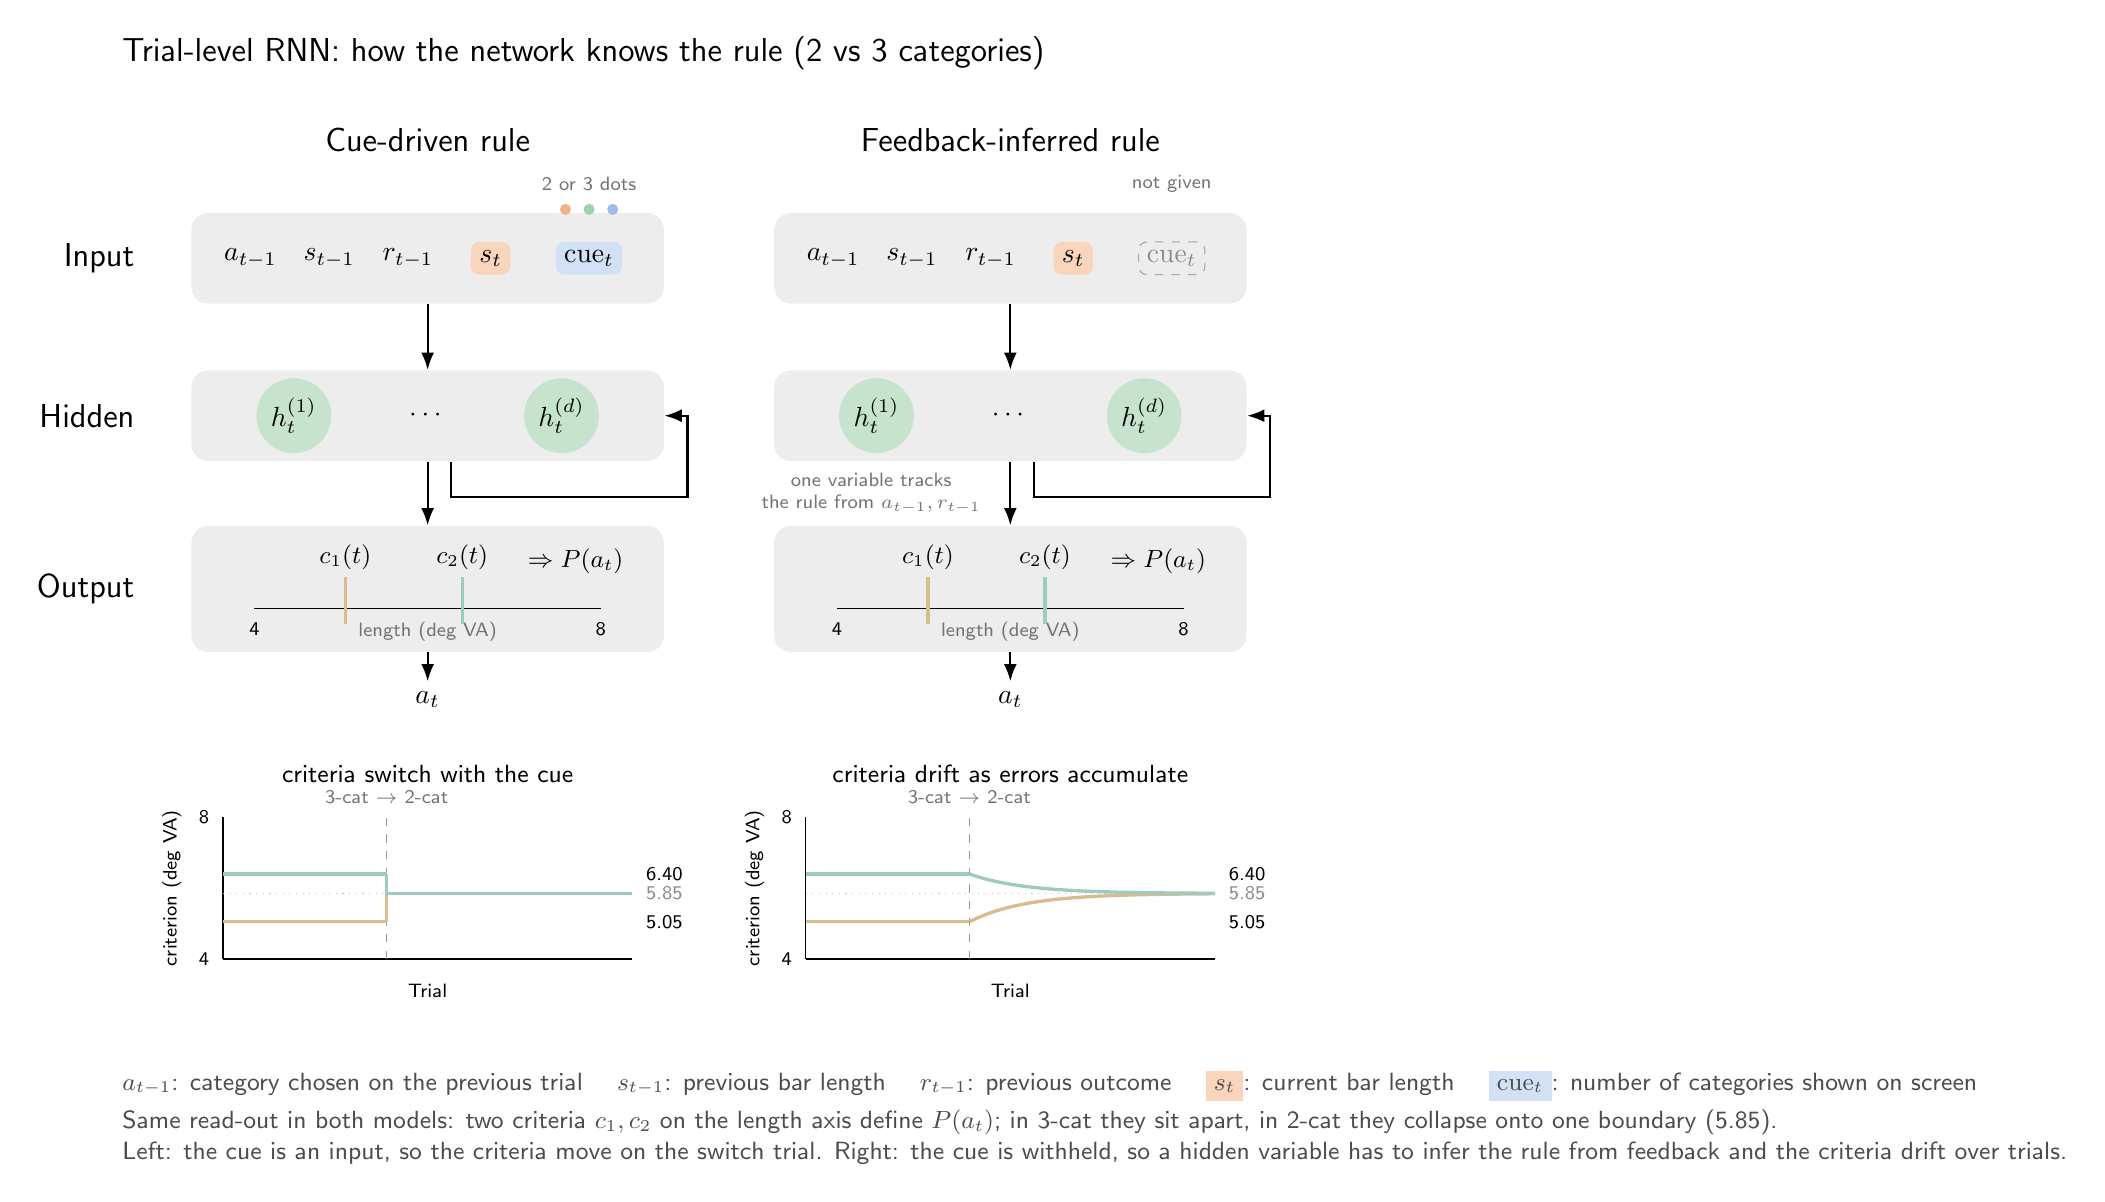
\begin{tikzpicture}[ctpanel,
  cue/.style={fill=catLong!45, rounded corners=3pt, inner sep=3pt},
  ghost/.style={draw=black!35, dashed, rounded corners=3pt, inner sep=3pt, text=black!45},
  crit/.style={line width=1.2pt},
  note/.style={font=\sffamily\scriptsize, text=black!55, align=center},
]

\node[font=\sffamily\large, anchor=west] at (-1.0,2.6)
  {Trial-level RNN: how the network knows the rule (2 vs 3 categories)};

\node[rowlab] at (-0.6, 0)   {Input};
\node[rowlab] at (-0.6,-2.0) {Hidden};
\node[rowlab] at (-0.6,-4.2) {Output};

% =============== LEFT: cue-driven rule ===============
\begin{scope}[xshift=0cm]
  \node[font=\sffamily\large] at (3.0, 1.5) {Cue-driven rule};
  \node[band, minimum width=6.0cm] (Lin) at (3.0,0) {};
  \node at (0.75,0) {$a_{t-1}$};
  \node at (1.75,0) {$s_{t-1}$};
  \node at (2.75,0) {$r_{t-1}$};
  \node[now] at (3.8,0) {$s_{t}$};
  \node[cue] (Lcue) at (5.05,0) {$\mathrm{cue}_t$};
  % cue icon: 3 dots / 2 dots above the token
  \fill[catShort] (4.75,0.62) circle (0.7mm);
  \fill[catMid]   (5.05,0.62) circle (0.7mm);
  \fill[catLong]  (5.35,0.62) circle (0.7mm);
  \node[note] at (5.05,0.95) {2 or 3 dots};

  \node[band, minimum width=6.0cm] (Lh) at (3.0,-2.0) {};
  \node[unit] at (1.3,-2.0) {$h_t^{(1)}$};
  \node at (3.0,-2.0) {$\cdots$};
  \node[unit] at (4.7,-2.0) {$h_t^{(d)}$};

  \node[band, minimum width=6.0cm, minimum height=1.6cm] (Lout) at (3.0,-4.2) {};
  % length axis with two criteria
  \draw[axis] (0.8,-4.45) -- (5.2,-4.45);
  \node[font=\sffamily\scriptsize, anchor=north] at (0.8,-4.5) {4};
  \node[font=\sffamily\scriptsize, anchor=north] at (5.2,-4.5) {8};
  \node[font=\sffamily\scriptsize, anchor=north, text=black!55] at (3.0,-4.5) {length (deg VA)};
  % 3-cat criteria at 5.05 and 6.40 mapped onto 0.8..5.2
  \draw[crit, catShort!70!catMid] (1.955,-4.65) -- (1.955,-4.05);
  \draw[crit, catMid!70!catLong]  (3.44,-4.65)  -- (3.44,-4.05);
  \node[font=\small] at (1.955,-3.8) {$c_1(t)$};
  \node[font=\small] at (3.44,-3.8)  {$c_2(t)$};
  \node[font=\small, anchor=west] at (4.15,-3.85) {$\Rightarrow P(a_t)$};
  \node (La) at (3.0,-5.6) {$a_t$};

  \draw[flow] (Lin.south) -- (Lh.north);
  \draw[flow] (Lh.south) -- (Lout.north);
  \draw[flow] (Lout.south) -- (La);
  \draw[flow] (Lh.south) ++(0.3,0) |- ++(3.0,-0.45) |- (Lh.east);
\end{scope}

% =============== RIGHT: feedback-inferred rule ===============
\begin{scope}[xshift=7.4cm]
  \node[font=\sffamily\large] at (3.0, 1.5) {Feedback-inferred rule};
  \node[band, minimum width=6.0cm] (Rin) at (3.0,0) {};
  \node at (0.75,0) {$a_{t-1}$};
  \node at (1.75,0) {$s_{t-1}$};
  \node at (2.75,0) {$r_{t-1}$};
  \node[now] at (3.8,0) {$s_{t}$};
  \node[ghost] at (5.05,0) {$\mathrm{cue}_t$};
  \node[note] at (5.05,0.95) {not given};

  \node[band, minimum width=6.0cm] (Rh) at (3.0,-2.0) {};
  \node[unit] at (1.3,-2.0) {$h_t^{(1)}$};
  \node at (3.0,-2.0) {$\cdots$};
  \node[unit] at (4.7,-2.0) {$h_t^{(d)}$};
  \node[note, anchor=north east] at (2.75,-2.6) {one variable tracks\\ the rule from $a_{t-1}, r_{t-1}$};

  \node[band, minimum width=6.0cm, minimum height=1.6cm] (Rout) at (3.0,-4.2) {};
  \draw[axis] (0.8,-4.45) -- (5.2,-4.45);
  \node[font=\sffamily\scriptsize, anchor=north] at (0.8,-4.5) {4};
  \node[font=\sffamily\scriptsize, anchor=north] at (5.2,-4.5) {8};
  \node[font=\sffamily\scriptsize, anchor=north, text=black!55] at (3.0,-4.5) {length (deg VA)};
  \draw[crit, catShort!70!catMid] (1.955,-4.65) -- (1.955,-4.05);
  \draw[crit, catMid!70!catLong]  (3.44,-4.65)  -- (3.44,-4.05);
  \node[font=\small] at (1.955,-3.8) {$c_1(t)$};
  \node[font=\small] at (3.44,-3.8)  {$c_2(t)$};
  \node[font=\small, anchor=west] at (4.15,-3.85) {$\Rightarrow P(a_t)$};
  \node (Ra) at (3.0,-5.6) {$a_t$};

  \draw[flow] (Rin.south) -- (Rh.north);
  \draw[flow] (Rh.south) -- (Rout.north);
  \draw[flow] (Rout.south) -- (Ra);
  \draw[flow] (Rh.south) ++(0.3,0) |- ++(3.0,-0.45) |- (Rh.east);
\end{scope}

% =============== BOTTOM: criteria across a block switch ===============
% y map: deg VA v -> (v-4)/4*1.8 ; x: trial 0..30, switch at trial 12
\newcommand{\critplot}[3]{%
  % #1 = xshift, #2 = title, #3 = "step" or "gradual"
  \begin{scope}[xshift=#1, yshift=-8.9cm]
    \draw[axis] (0,0) -- (0,1.8);
    \draw[axis] (0,0) -- (5.2,0);
    \node[font=\sffamily\scriptsize, rotate=90] at (-0.65,0.9) {criterion (deg VA)};
    \node[font=\sffamily\scriptsize] at (2.6,-0.4) {Trial};
    \node[font=\sffamily\scriptsize, anchor=east] at (-0.05,0.0) {4};
    \node[font=\sffamily\scriptsize, anchor=east] at (-0.05,1.8) {8};
    \draw[black!40, dashed] (2.08,0) -- (2.08,1.8);
    \node[font=\sffamily\scriptsize, text=black!55, anchor=south] at (2.08,1.85) {3-cat $\rightarrow$ 2-cat};
    % nominal 2-cat criterion 5.85 -> 0.8325 ; 3-cat 5.05 -> 0.4725, 6.40 -> 1.08
    \draw[black!25, dotted] (0,0.8325) -- (5.2,0.8325);
    \node[font=\sffamily\scriptsize, anchor=west, text=black!45] at (5.25,0.8325) {5.85};
    \node[font=\sffamily\scriptsize, anchor=west] at (5.25,0.4725) {5.05};
    \node[font=\sffamily\scriptsize, anchor=west] at (5.25,1.08)   {6.40};
    \draw[crit, catShort!70!catMid] (0,0.4725) -- (2.08,0.4725);
    \draw[crit, catMid!70!catLong]  (0,1.08)   -- (2.08,1.08);
    \ifnum\pdfstrcmp{#3}{step}=0
      \draw[crit, catShort!70!catMid] (2.08,0.4725) -- (2.08,0.8325) -- (5.2,0.8325);
      \draw[crit, catMid!70!catLong]  (2.08,1.08)   -- (2.08,0.8325) -- (5.2,0.8325);
    \else
      \draw[crit, catShort!70!catMid, domain=2.08:5.2, samples=60, smooth]
        plot (\x, {0.8325 - 0.36*exp(-(\x-2.08)/0.7)});
      \draw[crit, catMid!70!catLong,  domain=2.08:5.2, samples=60, smooth]
        plot (\x, {0.8325 + 0.2475*exp(-(\x-2.08)/0.7)});
    \fi
    \node[font=\sffamily\small] at (2.6,2.35) {#2};
  \end{scope}
}
\critplot{0.4cm}{criteria switch with the cue}{step}
\critplot{7.8cm}{criteria drift as errors accumulate}{gradual}

% =============== legend ===============
\node[align=left, anchor=north west, font=\sffamily\small, text=black!70] at (-1.0,-10.2) {%
  $a_{t-1}$: category chosen on the previous trial \quad
  $s_{t-1}$: previous bar length \quad
  $r_{t-1}$: previous outcome \quad
  \colorbox{catShort!55}{$s_t$}: current bar length \quad
  \colorbox{catLong!45}{$\mathrm{cue}_t$}: number of categories shown on screen\\[3pt]
  Same read-out in both models: two criteria $c_1, c_2$ on the length axis define $P(a_t)$;
  in 3-cat they sit apart, in 2-cat they collapse onto one boundary (5.85).\\
  Left: the cue is an input, so the criteria move on the switch trial. Right: the cue is
  withheld, so a hidden variable has to infer the rule from feedback and the criteria
  drift over trials.
};

\end{tikzpicture}
\end{document}
